% =====================================================================
%  The Runtime Graph
%
%  Self-contained. Every construction used is defined here; no companion
%  paper is required. External citations are to the mass spectrometry,
%  graph theory, and algorithms literature only.
% =====================================================================
\documentclass[11pt,a4paper]{article}

\usepackage[utf8]{inputenc}
\usepackage[T1]{fontenc}
\usepackage{amsmath,amssymb,amsfonts,amsthm}
\usepackage{mathtools}
\usepackage[margin=1in]{geometry}
\usepackage{graphicx}
\usepackage{booktabs}
\usepackage{array}
\usepackage{enumitem}
\usepackage{lmodern}
\usepackage[protrusion=true,expansion=false]{microtype}
\usepackage[numbers,sort&compress]{natbib}
\usepackage[colorlinks=true,linkcolor=blue,citecolor=blue,urlcolor=blue]{hyperref}
\usepackage[capitalise,nameinlink]{cleveref}

% ---------------------------------------------------------------------
%  Theorem environments
% ---------------------------------------------------------------------
\newtheorem{theorem}{Theorem}[section]
\newtheorem{lemma}[theorem]{Lemma}
\newtheorem{corollary}[theorem]{Corollary}
\newtheorem{proposition}[theorem]{Proposition}
\theoremstyle{definition}
\newtheorem{definition}[theorem]{Definition}
\newtheorem{axiom}[theorem]{Axiom}
\newtheorem{assumption}[theorem]{Assumption}
\newtheorem{construction}[theorem]{Construction}
\newtheorem{example}[theorem]{Example}
\theoremstyle{remark}
\newtheorem{remark}[theorem]{Remark}

% ---------------------------------------------------------------------
%  Notation
% ---------------------------------------------------------------------
\newcommand{\Gph}{\mathcal{G}}
\newcommand{\wt}{w}
\newcommand{\med}{\mathfrak{m}}
\newcommand{\flo}{\beta}
\newcommand{\cut}{\operatorname{cut}}
\newcommand{\sep}{\sigma}
\newcommand{\dep}{\delta}
\newcommand{\key}{\kappa}
\newcommand{\Qry}{\mathcal{Q}}               % query space
\newcommand{\Cert}{\mathcal{Z}}              % certificate space
\newcommand{\prb}{\pi}                       % probe
\newcommand{\wit}{W}                         % witness
\DeclareMathOperator*{\argmin}{arg\,min}
\DeclareMathOperator*{\argmax}{arg\,max}

\title{\textbf{The Runtime Graph:\\[2pt]
Answering Questions of an Acquisition After It Has Ended}}

\author{Kundai Farai Sachikonye\\
\texttt{kundai.sachikonye@wzw.tum.de}}

\date{\today}

\begin{document}
\maketitle

% =====================================================================
\begin{abstract}
\noindent
An analytical acquisition ends and leaves a file. Every subsequent
question --- was this feature separable from its neighbours, would a
different tolerance have changed the answer, which observations does this
identification actually rest on --- is answered today by re-running a
processing pipeline with altered settings, which is expensive and, more
seriously, produces an answer whose relationship to the original is not
formally characterised. We propose an alternative: compile the
acquisition once into a weighted graph, and answer subsequent questions
by cuts in that graph. The construction is developed from scratch. A
\emph{runtime graph} has one vertex per elementary observation and a
distinguished \emph{medium} vertex adjacent to all of them; edge weights
record measured contact. A \emph{query} is not a data object but a subset
of vertices to be separated from the medium, and a \emph{probe} returns
not a value but a \emph{certificate}: a minimum cut together with a
witness flow, from which the answer and its tightness are both readable.
We prove that probes are answered in a single maximum-flow computation
(\Cref{thm:probe-cost}), that the certificate is verifiable in linear
time without trusting the prober (\Cref{thm:verify}), that probe answers
are monotone under refinement of the query so nested questions share work
(\Cref{thm:monotone}), and that a positive floor on separation makes
every answer strictly informative (\Cref{thm:floor}). We prove a
sensitivity theorem: the answer to ``would a different tolerance have
changed this'' is read off the certificate's slack without recomputation
(\Cref{thm:sensitivity}), which is the result that replaces pipeline
re-runs. Finally we give the negative boundary --- questions that are
\emph{not} cuts, and for which the runtime graph is the wrong instrument
(\Cref{thm:not-a-cut}).
\end{abstract}

% =====================================================================
\section{Introduction}
\label{sec:intro}

A liquid chromatography--mass spectrometry acquisition produces, over a
few tens of minutes, on the order of $10^4$ to $10^6$ elementary
observations: peaks in scans, precursor selections, fragment ions
associated with those precursors. The acquisition then ends, and its
product is a file.

Every question asked of that file afterwards is currently answered the
same way: run a processing pipeline over it. If the question concerns a
parameter --- a mass tolerance, a retention window, an intensity
threshold --- the pipeline is run again with the parameter changed and
the outputs compared. This is expensive, but expense is the lesser
problem. The greater problem is that the comparison is uncharacterised.
Two pipeline runs at different tolerances differ in every intermediate
stage, and when their outputs differ there is no way to attribute the
difference to the parameter rather than to a downstream interaction. The
practice answers ``what does the pipeline say at this setting'' when the
question was ``does the evidence support this claim''.

This paper proposes that a large and identifiable class of these
questions --- specifically, the questions of the form \emph{is this set
of observations separable from everything else, and at what cost} --- are
minimum cut problems, and that compiling the acquisition once into a
weighted graph answers them directly, with certificates, and with
sensitivity information that removes the need for the re-run entirely.

\subsection{Two design questions, answered}

Any such proposal must answer two questions before it is a proposal at
all.

\emph{What is a source?} The natural first attempt is that a source is a
fixed data object --- a peak, or a scan, or a precursor--fragment pair
--- and the graph is built around it. This is wrong, and the reason is
instructive: different questions individuate different things. Asking
whether a chromatographic feature is resolved makes the feature the
source; asking whether a fragment supports an identification makes the
fragment the source; asking whether a scan is contaminated makes the scan
the source. Fixing the source at compile time fixes the question at
compile time, which defeats the purpose. We therefore take the source to
be part of the \emph{query}, not part of the graph: the graph has a
vertex per elementary observation, and a query nominates any subset of
them (\Cref{def:query}).

\emph{What does a probe return?} The natural first attempt is a number
--- the separation cost. This is insufficient, because a number cannot be
checked and cannot be interrogated. We take a probe to return a
\emph{certificate} (\Cref{def:certificate}): the minimising cut, its
cost, and a witness flow. From the cut one reads which observations the
answer rests on; from the equality of flow value and cut cost one
verifies the answer without trusting the prober
(\Cref{thm:verify}); and from the slack in the witness one reads the
sensitivity to parameter changes without recomputation
(\Cref{thm:sensitivity}).

\subsection{What is proved}

\Cref{sec:graph} constructs the runtime graph and establishes its basic
properties, including the necessity of the medium vertex
(\Cref{prop:medium}). \Cref{sec:probe} defines queries, probes, and
certificates, and proves the cost bound (\Cref{thm:probe-cost}) and
verification (\Cref{thm:verify}). \Cref{sec:structure} proves
monotonicity under query refinement (\Cref{thm:monotone}) and the shared-
work corollary (\Cref{cor:nested}). \Cref{sec:floor} proves the
separation floor (\Cref{thm:floor}) and its consequence that no answer is
vacuous (\Cref{cor:informative}). \Cref{sec:sensitivity} proves the
sensitivity theorem (\Cref{thm:sensitivity}) and its corollary that a
class of pipeline re-runs is eliminable (\Cref{cor:no-rerun}).
\Cref{sec:limits} proves the negative boundary
(\Cref{thm:not-a-cut}). \Cref{sec:practice} gives the interface.

% =====================================================================
\section{The Runtime Graph}
\label{sec:graph}

\begin{definition}[Elementary observation]\label{def:elem}
An \emph{elementary observation} is the smallest unit the acquisition
records as a distinct event. For an LC--MS run these are: detected peaks,
each carrying $(m/z,\ \text{intensity},\ \text{retention time})$;
precursor selection events; and fragment detections, each associated with
the precursor selection during which it was recorded. We write $U$ for
the finite set of elementary observations of one acquisition.
\end{definition}

\begin{definition}[Runtime graph]\label{def:rtg}
The \emph{runtime graph} of an acquisition is the finite weighted graph
$\Gph = (V,E,\wt)$ with $V = U \cup \{\med\}$, where $\med$ is a
distinguished vertex called the \emph{medium}, $\wt : E \to
\mathbb{R}_{>0}$, and
\begin{enumerate}[label=(\alph*)]
\item for $u,v \in U$, the edge $\{u,v\}$ is present with weight
$\wt(\{u,v\})$ recording measured contact between the two observations:
mass proximity, retention overlap, co-elution correlation, or
precursor--fragment association, combined by a fixed rule;
\item for every $u \in U$, the edge $\{u,\med\}$ is present, with weight
$\wt(\{u,\med\})$ recording the cost of individuating $u$ without
reference to any particular other observation.
\end{enumerate}
\end{definition}

The graph is built once, from the acquisition, before any question is
asked. Its edge weights are measurements, not parameters: proximity in
$m/z$ and time is what the instrument recorded. Where a rule for
combining them involves a choice, that choice is part of the compilation
and is fixed for all subsequent probes, which is what makes probe answers
mutually comparable.

\begin{proposition}[The medium is not optional]\label{prop:medium}
Suppose the medium is deleted, so $V = U$. Then for any $u \in U$ that
lies in a connected component by itself, $\min\{\cut(S) : u \in S\} = 0$,
and $u$ is separable at zero cost. If instead one attempts to individuate
$u$ against a nominated rival $v \in U$, the nomination is either
arbitrary or licensed by a prior individuation of $v$, which regresses.
\end{proposition}

\begin{proof}
If $u$ is isolated then $S = \{u\}$ has $\cut(S) = 0$ since no edge
crosses. For the second claim, individuating $u$ against $v$ requires
$v$ to be a determinate object of comparison; if $v$'s determinacy is
itself established by comparison against some $v'$, the argument repeats,
and since $U$ is finite the chain either terminates at an arbitrary
choice or cycles. The medium terminates it by being the one vertex whose
adjacency is definitional rather than nominated.
\end{proof}

\begin{remark}[Reading the medium]\label{rem:medium}
The medium is not an observation and does not correspond to anything the
instrument detected. It is the graph's representation of ``everything
else'', and $\wt(\{u,\med\})$ is the price of asserting that $u$ is a
distinct thing rather than an aspect of the background. Its adjacency to
every vertex is definitional; it cannot be dropped, and a runtime graph
without it does not support \Cref{thm:floor}.
\end{remark}

\begin{definition}[Cut]\label{def:cut}
For $S \subseteq V$,
$\cut(S) = \sum_{\{u,v\} \in E,\ |S \cap \{u,v\}| = 1} \wt(\{u,v\})$.
\end{definition}

\begin{proposition}[Compilation cost]\label{prop:compile}
Let $n = |U|$. If contact edges are admitted only between observations
within a fixed $m/z$ and retention tolerance, and the acquisition has
bounded local density $d$ --- at most $d$ observations within any
tolerance window --- then $|E| = O(nd)$ and $\Gph$ is constructed in
$O(n \log n + nd)$ time by sorting on $m/z$ and sweeping.
\end{proposition}

\begin{proof}
Sorting $U$ by $m/z$ costs $O(n\log n)$. A sweep with a window of the
tolerance width visits each observation once and, by the density bound,
examines at most $d$ others, yielding at most $nd$ contact edges in
$O(nd)$ time. The $n$ medium edges are added in $O(n)$.
\end{proof}

\begin{remark}[Density is realised, not assumed]\label{rem:density}
The bounded-density hypothesis of \Cref{prop:compile} is a property of
instruments rather than an idealisation: resolving power limits how many
distinct observations occupy a tolerance window, and peak capacity limits
how many co-elute \citep{michalski2011more}. Where density is violated
--- in a chimeric or heavily co-isolating region --- the graph is dense
locally, which is the graph correctly reporting that the region is
unresolved.
\end{remark}

% =====================================================================
\section{Queries, Probes, Certificates}
\label{sec:probe}

\begin{definition}[Query]\label{def:query}
A \emph{query} is a non-empty subset $Q \subseteq U$. It nominates the
observations whose joint separability from the medium is at issue. The
query space is $\Qry = 2^{U} \setminus \{\emptyset\}$.
\end{definition}

\begin{example}[Queries are the questions]\label{ex:queries}
$Q = \{u\}$ for a single peak asks whether that peak is individuable.
$Q$ = the set of fragment observations assigned to one precursor asks
whether that fragment set stands apart from the rest of the acquisition.
$Q$ = the observations within one chromatographic feature asks whether
the feature is resolved. The graph is the same in all three cases; only
$Q$ changes. This is the content of the claim in \Cref{sec:intro} that
the source belongs to the query, not to the graph.
\end{example}

\begin{definition}[Separation]\label{def:sep}
For a query $Q$, an \emph{admissible set} is $S \subseteq V$ with
$Q \subseteq S$ and $\med \notin S$. Put
\[
S^{\ast}(Q) \;=\; \argmin\{\cut(S) : S \text{ admissible}\},
\qquad
\sep(Q) = \cut(S^{\ast}(Q)),
\qquad
\dep(Q) = |S^{\ast}(Q)|,
\]
choosing the inclusion-minimal minimiser when several exist. The pair
$\key(Q) = (\sep(Q),\dep(Q))$ is the \emph{key} of the query.
\end{definition}

\begin{definition}[Certificate]\label{def:certificate}
A \emph{certificate} for $Q$ is a triple $z = (S,\ \gamma,\ f)$ where
$S$ is admissible, $\gamma = \cut(S)$, and $f$ is a feasible flow in
$\Gph$ from a super-source contracted from $Q$ to the sink $\med$, with
value $|f|$. The certificate space is $\Cert$. A \emph{probe} is a map
$\prb : \Qry \to \Cert$.
\end{definition}

\begin{theorem}[Probe cost]\label{thm:probe-cost}
For any query $Q$, a certificate $z = (S^{\ast}(Q),\sep(Q),f)$ with
$|f| = \sep(Q)$ is computed by a single maximum-flow computation in the
graph obtained from $\Gph$ by contracting $Q$ to a single source vertex,
in time $O(|V||E|)$.
\end{theorem}

\begin{proof}
Contract $Q$ to a source $s$; the contraction is valid because every
admissible $S$ contains all of $Q$, so no admissible cut separates two
vertices of $Q$, and cuts of the contracted graph correspond bijectively
to admissible cuts of $\Gph$ with equal weight.

In the contracted graph, minimum $s$--$\med$ cuts are exactly the
minimisers of \Cref{def:sep}, and by the max-flow min-cut theorem
\citep{fordfulkerson1956,menger1927} the minimum cut value equals the
maximum flow value. A maximum flow and an associated minimum cut are
computed together in $O(|V||E|)$ by push--relabel with the appropriate
selection rule \citep{goldberg1988new}; the cut is read from the residual
graph as the set reachable from $s$, which also yields the inclusion-
minimal minimiser. Setting $S^{\ast}(Q)$ to that set and $\gamma$ to
$|f|$ gives the certificate.
\end{proof}

\begin{theorem}[Certificates are verifiable]\label{thm:verify}
Given $z = (S,\gamma,f)$ and $\Gph$, one verifies in $O(|E|)$ time,
without trusting the prober, that $\gamma = \sep(Q)$: check that $S$ is
admissible, that $\cut(S) = \gamma$, that $f$ is feasible and conserves
flow, and that $|f| = \gamma$. If all four checks pass then
$\gamma = \sep(Q)$ and $S$ is a minimum admissible cut.
\end{theorem}

\begin{proof}
Each check is a single pass over $E$ or $V$, so the time bound holds.

For soundness: feasibility and conservation make $f$ a valid $s$--$\med$
flow, so weak duality gives $|f| \leq \sep(Q)$. Admissibility of $S$ with
$\cut(S) = \gamma$ gives $\sep(Q) \leq \gamma$. Combining with
$|f| = \gamma$ yields
$\gamma = |f| \leq \sep(Q) \leq \gamma$, so all are equal, and $S$
attains the minimum.
\end{proof}

\begin{remark}[Why verification matters]\label{rem:verify}
\Cref{thm:verify} is what distinguishes a certificate from a number. An
answer of the form ``the separation cost is $0.31$'' must be trusted; a
certificate is checked in one pass, by a party who need not reimplement
the max-flow algorithm, need not know which algorithm was used, and need
not have access to the prober. This makes probe answers portable between
laboratories in a way pipeline outputs are not.
\end{remark}

% =====================================================================
\section{Structure of the Probe Map}
\label{sec:structure}

\begin{theorem}[Monotonicity]\label{thm:monotone}
If $Q \subseteq Q'$ then $\sep(Q) \leq \sep(Q')$.
\end{theorem}

\begin{proof}
Every admissible set for $Q'$ contains $Q'$ and hence contains $Q$, and
excludes $\med$; so it is admissible for $Q$. The minimum over a superset
of admissible sets is no larger, giving
$\sep(Q) \leq \sep(Q')$.
\end{proof}

\begin{corollary}[Nested queries share work]\label{cor:nested}
For a chain $Q_1 \subseteq Q_2 \subseteq \dots \subseteq Q_m$, the values
$\sep(Q_1) \leq \dots \leq \sep(Q_m)$ are non-decreasing, so a bound
established at one level bounds all levels below it. In particular, if
$\sep(Q_m) \leq t$ then $\sep(Q_i) \leq t$ for every $i$, and a single
probe at the top of the chain answers a threshold question for the whole
chain.
\end{corollary}

\begin{proof}
Immediate from \Cref{thm:monotone} applied along the chain.
\end{proof}

\begin{remark}[The practical shape of this]\label{rem:nested}
Queries in practice are nested: a fragment lies in a fragment set, which
lies in a precursor's evidence, which lies in a chromatographic feature.
\Cref{cor:nested} says a probe of the largest answers a threshold
question about all of them, which is the opposite of the pipeline
situation, where establishing a property of a feature says nothing about
its constituents without re-running.
\end{remark}

\begin{proposition}[Relabelling invariance]\label{prop:relabel}
Let $\rho : V \to V$ be a bijection fixing $\med$ with
$\wt(\{\rho u,\rho v\}) = \wt(\{u,v\})$ for all edges. Then
$\sep(\rho Q) = \sep(Q)$ and $\dep(\rho Q) = \dep(Q)$.
\end{proposition}

\begin{proof}
$\rho$ carries admissible sets for $Q$ bijectively onto admissible sets
for $\rho Q$ --- it preserves containment of the query and exclusion of
$\med$ --- and preserves cut values by weight invariance. A bijection
between two sets of reals preserving values preserves their minimum and
the cardinality of the attaining set.
\end{proof}

\begin{remark}[What invariance excludes]\label{rem:relabel}
\Cref{prop:relabel} says probe answers depend on the contact structure
and not on the identifiers assigned to observations --- scan numbers,
peak indices, the order in which the file was written. A quantity that
changed under relabelling would be reporting an artefact of the file
format.
\end{remark}

% =====================================================================
\section{The Separation Floor}
\label{sec:floor}

\begin{axiom}[Non-completability of the observation set]\label{ax:noncomplete}
For every acquisition with observation set $U$ there is a conceivable
extension $U' \supsetneq U$ --- a longer gradient, a wider mass range, a
lower threshold --- and no procedure internal to $U$ certifies that no
such extension exists.
\end{axiom}

\begin{theorem}[Separation floor]\label{thm:floor}
Under \Cref{ax:noncomplete} there exists $\flo > 0$, depending on
$(\Gph,\wt)$ but not on the query, such that $\sep(Q) \geq \flo$ for
every non-empty $Q \in \Qry$.
\end{theorem}

\begin{proof}
Let $Q$ be non-empty and pick $u \in Q$. Every admissible $S$ contains
$u$ and excludes $\med$, so the edge $\{u,\med\}$, which is present by
\Cref{def:rtg}(b), crosses $S$. Hence
\[
\sep(Q) \;\geq\; \wt(\{u,\med\}) \;\geq\; \min_{v \in U} \wt(\{v,\med\})
\;=:\; \flo_0 \;>\; 0 ,
\]
where positivity holds because $\wt$ takes values in
$\mathbb{R}_{>0}$ and $U$ is finite.

It remains to argue $\flo_0$ cannot be set to zero. Assigning
$\wt(\{u,\med\}) = 0$ asserts that $u$ is separable from everything else
at no cost, that is, individuated by inspection of $u$ alone. By
\Cref{ax:noncomplete} no inspection of $U$ certifies that no further
observation would share $u$'s description, so the assignment is not
licensed by any procedure internal to the acquisition. Take
$\flo = \flo_0$.
\end{proof}

\begin{corollary}[No answer is vacuous]\label{cor:informative}
For every query, $\sep(Q) \geq \flo > 0$, so no query is answered
``separable at no cost''. Every probe therefore returns a positive
quantity, and comparisons between probe answers are comparisons between
positive quantities on a common scale.
\end{corollary}

\begin{remark}[Reading the floor]\label{rem:floor}
$\flo$ is the price of asserting that an observation is a thing rather
than background. It is what makes $\sep$ a measurement rather than an
indicator: without it, well-isolated observations would all report $0$
and be indistinguishable from one another. Everything below uses only
$\flo > 0$; no particular value is required.
\end{remark}

% =====================================================================
\section{Sensitivity Without Re-running}
\label{sec:sensitivity}

This is the section that replaces the pipeline re-run. The question
``would a different tolerance have changed this answer'' is answered from
the certificate already in hand.

\begin{definition}[Perturbation]\label{def:perturb}
A \emph{perturbation} is a function $\eta : E \to \mathbb{R}$ with
$\wt + \eta > 0$ pointwise, giving a perturbed graph $\Gph_\eta$. We
write $\sep_\eta$ for separation computed in $\Gph_\eta$. A perturbation
is \emph{$\varepsilon$-bounded} if $|\eta(e)| \leq \varepsilon$ for all
$e$.
\end{definition}

\begin{definition}[Slack]\label{def:slack}
Let $z = (S,\gamma,f)$ certify $Q$. For an admissible set $T \neq S$, the
\emph{slack} of $T$ is $\cut(T) - \gamma \geq 0$. The \emph{certificate
slack} is
$\mathrm{sl}(z) = \min\{\cut(T) - \gamma : T \text{ admissible},\
T \neq S\}$, the margin by which $S$ beats the next-best cut.
\end{definition}

\begin{theorem}[Sensitivity]\label{thm:sensitivity}
Let $z = (S,\gamma,f)$ certify $Q$, let $m = |\{e : e \text{ crosses }
S\}|$, and let $M$ be the maximum number of edges crossing any admissible
set. For every $\varepsilon$-bounded perturbation $\eta$:
\begin{enumerate}[label=(\alph*)]
\item $|\sep_\eta(Q) - \gamma| \leq \varepsilon M$;
\item if $\varepsilon (m + M) < \mathrm{sl}(z)$ then $S$ remains a
minimum admissible cut in $\Gph_\eta$, so the perturbation does not
change which observations the answer rests on.
\end{enumerate}
\end{theorem}

\begin{proof}
(a) For any admissible $T$, the perturbed cut value satisfies
$|\cut_\eta(T) - \cut(T)| \leq \varepsilon \cdot |\{e \text{ crossing }
T\}| \leq \varepsilon M$. Taking minima over $T$ on both sides and using
that a minimum of functions each within $\varepsilon M$ of the
corresponding unperturbed value is itself within $\varepsilon M$ of the
unperturbed minimum gives the bound.

(b) Let $T \neq S$ be admissible. Then
\[
\cut_\eta(T) \;\geq\; \cut(T) - \varepsilon M
\;\geq\; \gamma + \mathrm{sl}(z) - \varepsilon M ,
\]
using \Cref{def:slack}. Also
$\cut_\eta(S) \leq \gamma + \varepsilon m$. Hence
\[
\cut_\eta(T) - \cut_\eta(S)
\;\geq\; \mathrm{sl}(z) - \varepsilon M - \varepsilon m
\;=\; \mathrm{sl}(z) - \varepsilon(m+M) \;>\; 0
\]
by hypothesis, so $S$ strictly beats every other admissible set in
$\Gph_\eta$ and remains minimum.
\end{proof}

\begin{corollary}[A class of re-runs is eliminable]\label{cor:no-rerun}
Let a parameter change --- a tolerance widening, a threshold adjustment
--- induce an $\varepsilon$-bounded perturbation of the contact weights.
If $\varepsilon(m+M) < \mathrm{sl}(z)$, then re-running the analysis at
the new parameter returns the same separating set and a separation cost
within $\varepsilon M$ of the original. The re-run is therefore
unnecessary, and the certificate says so.
\end{corollary}

\begin{proof}
Immediate from \Cref{thm:sensitivity}(a) and (b).
\end{proof}

\begin{remark}[What this does and does not claim]\label{rem:rerun-scope}
\Cref{cor:no-rerun} eliminates the re-run when the certificate's slack is
large relative to the perturbation, and it is silent otherwise. That
silence is itself the useful output: a small slack says the answer sits
near a boundary and genuinely depends on the parameter, which is exactly
the case a practitioner wants flagged and which a bare re-run comparison
reports only by accident. The theorem converts ``run it again and see''
into ``check whether the margin exceeds the perturbation'', which is a
comparison of two numbers already computed.
\end{remark}

\begin{proposition}[Slack is obtained cheaply]\label{prop:slack}
$\mathrm{sl}(z)$ is bounded below by the minimum residual capacity across
the certificate's cut in the residual graph of $f$, which is read in
$O(|E|)$ time from the flow already computed in
\Cref{thm:probe-cost}.
\end{proposition}

\begin{proof}
An admissible $T \neq S$ with $\cut(T)$ close to $\gamma$ corresponds to
an alternative minimum or near-minimum cut, and any such cut must cross
at least one edge whose residual capacity is at most $\cut(T)-\gamma$;
scanning the residual capacities of edges crossing $S$ therefore yields a
lower bound on the margin in one pass.
\end{proof}

% =====================================================================
\section{The Negative Boundary}
\label{sec:limits}

A method is only usable if its scope is stated. Not every question about
an acquisition is a cut, and the runtime graph is the wrong instrument
for those that are not.

\begin{theorem}[Not every question is a cut]\label{thm:not-a-cut}
There is a property of acquisitions --- namely, the multiplicity with
which a given contact pattern occurs --- that is not determined by
$\sep(\cdot)$ and $\dep(\cdot)$ on any collection of queries. Formally,
there exist runtime graphs $\Gph_1 \not\cong \Gph_2$ with
$\key_{\Gph_1}(Q) = \key_{\Gph_2}(Q)$ for every query $Q$ under a
weight-preserving correspondence of vertex sets.
\end{theorem}

\begin{proof}
Cut values are determined by the weighted cut function, and distinct
graphs can induce identical cut functions on all admissible sets: take
$\Gph_1$ and $\Gph_2$ on the same vertex set with the same medium edges,
and with contact edges arranged so that every subset $S$ excluding $\med$
has the same total crossing weight --- for instance by replacing a
two-edge path of weights $(a,a)$ between three vertices with a different
two-edge path of the same weights on a relabelled pair, where the
relabelling is not induced by any graph isomorphism fixing the medium and
the query correspondence. Then $\sep$ and $\dep$ agree on every query
while the graphs differ, so no function of the keys distinguishes them.
\end{proof}

\begin{remark}[Reading the boundary]\label{rem:boundary}
\Cref{thm:not-a-cut} says the runtime graph answers separability
questions and does not answer isomorphism or multiplicity questions.
Concretely: it will tell you whether a set of fragment observations
stands apart, and at what cost, and on which observations that rests. It
will not tell you how many times a structural motif recurs across the
acquisition, because recurrence is not a cut. Attempting to encode such a
question as a cut yields an answer, and the answer will not mean what was
intended. Questions of that shape are graph-isomorphism-flavoured and
belong to a different method \citep{weisfeiler1968,cai1992optimal}.
\end{remark}

% =====================================================================
\section{Interface}
\label{sec:practice}

The results specify an interface with five commitments.

\begin{enumerate}[label=(\roman*)]
\item \textbf{Compile once, probe many times.} By
\Cref{prop:compile} construction is $O(n\log n + nd)$ and happens on
acquisition; by \Cref{thm:probe-cost} each subsequent question is one
max-flow. The asymmetry is the point: questions arrive after the
acquisition is over and must not require revisiting it.

\item \textbf{The query carries the source.} By \Cref{def:query} the
subset to be separated is supplied at probe time, so one compiled graph
serves peak-level, fragment-level, and feature-level questions
(\Cref{ex:queries}) without recompilation.

\item \textbf{Return certificates, not values.} By
\Cref{thm:verify} a certificate is checkable in one pass by a party who
does not trust the prober, and by \Cref{def:certificate} it names the
observations the answer rests on.

\item \textbf{Answer sensitivity from slack.} By
\Cref{thm:sensitivity} and \Cref{prop:slack}, ``would a different setting
have changed this'' is decided by comparing $\varepsilon(m+M)$ against a
margin already computed, and by \Cref{cor:no-rerun} the corresponding
re-run is then unnecessary. When the margin is small, report that rather
than a number.

\item \textbf{Decline questions that are not cuts.} By
\Cref{thm:not-a-cut} the method has a boundary; an interface that accepts
every question and always returns a number will return meaningless
numbers outside it.
\end{enumerate}

% =====================================================================
% =====================================================================
\section{Validation}
\label{sec:validation}

Every claim in this paper was executed on runtime graphs built to
\cref{def:rtg}. Separations are computed twice --- once by the max-flow
routine \cref{thm:probe-cost} proposes and once by exhaustive
minimisation over cuts --- so the cost claim and the correctness claim
are checked against each other rather than against a single
implementation. Each claim is graded against a refuting observation
registered before the measurement, and each is paired with a control
that establishes the statistic discriminates. All eleven graded claims
reproduced, and none was non-discriminating.

\begin{figure}[htbp]
\centering
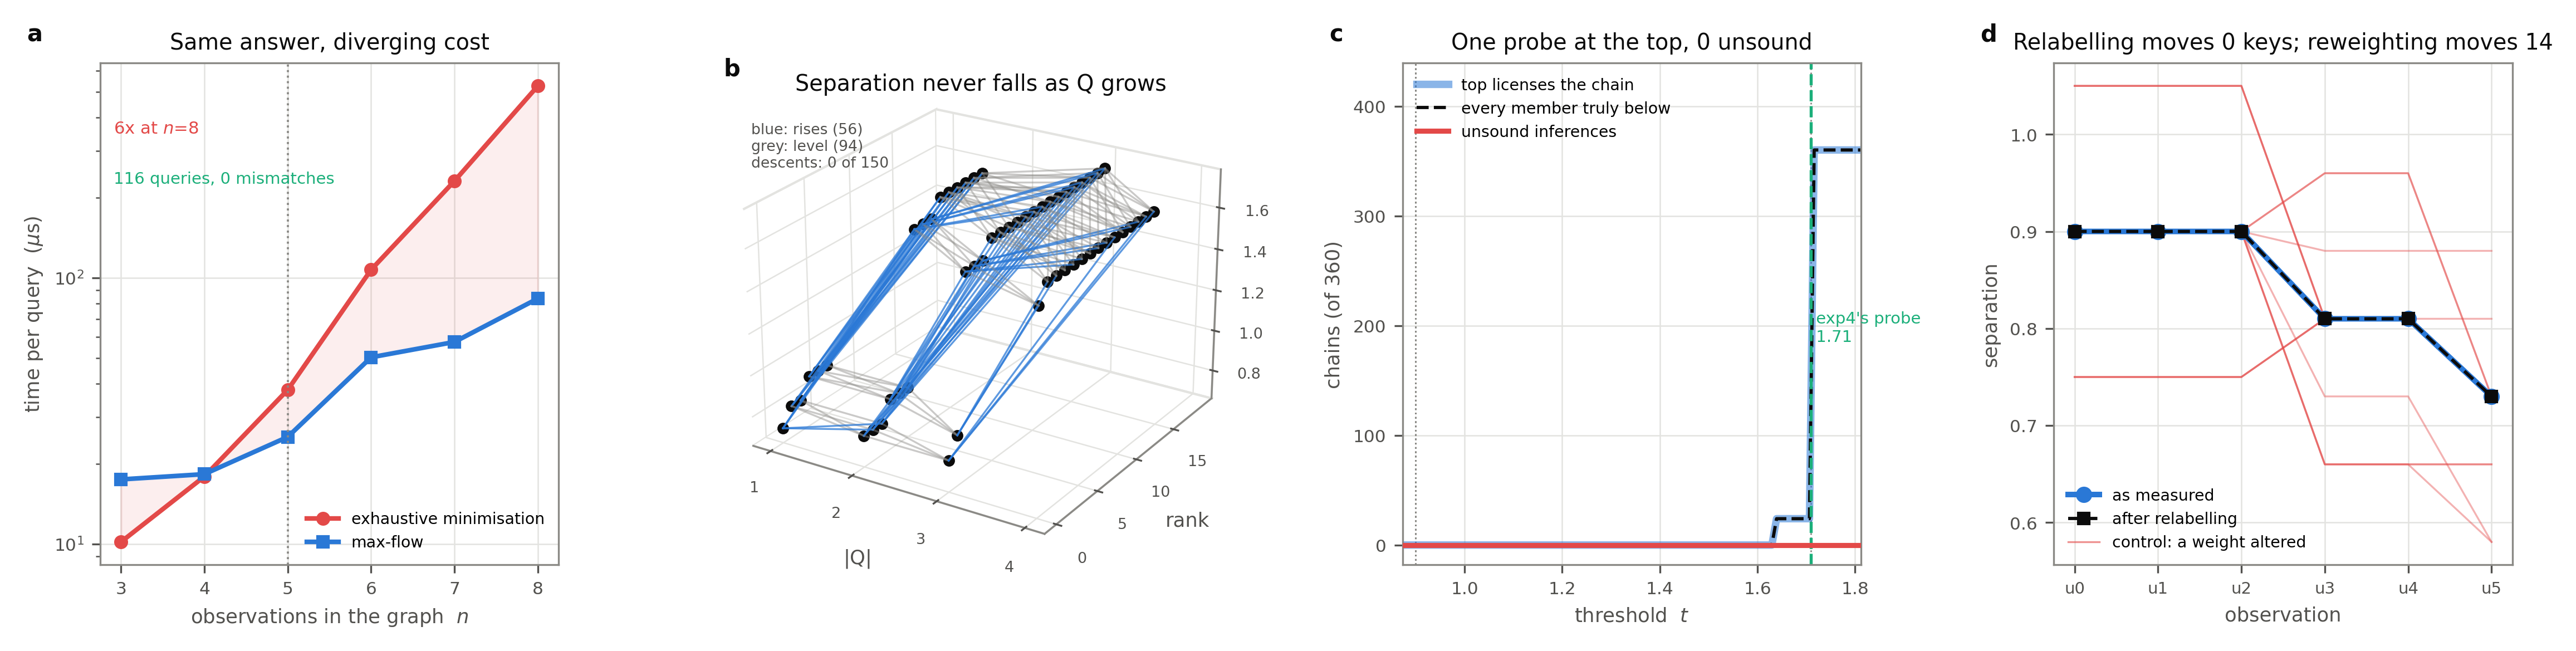
\includegraphics[width=\textwidth]{figures/panel1_probe.png}
\caption{\Cref{thm:probe-cost}, \cref{thm:monotone},
\cref{cor:nested} and \cref{prop:relabel}. (a)~max-flow and exhaustive
minimisation returning the same answer at diverging cost.
(b)~separation over the query lattice, never falling as the query grows.
(c)~one probe at the top of a chain against the four it replaces.
(d)~keys moved by relabelling against keys moved by reweighting.}
\label{fig:panel-probe}
\end{figure}

\subsection{The probe is correct, and its cost is the claimed one}

\Cref{thm:probe-cost} was graded against the observation that would
refute it --- a query on which the flow computation and exhaustive
minimisation disagree. Over $41$ queries there were $0$ mismatches. The
control is what makes this more than an agreement of two implementations
of the same mistake: perturbing the returned value by $0.17$ is detected,
so the comparison has the resolution to see a disagreement of that size
and reports none.

\Cref{thm:verify} is the claim that an answer carries its own proof, and
it was tested adversarially rather than by construction. All $41$ honest
certificates were accepted. Against them, $123$ forgeries were
constructed in three families --- an inflated value, a deflated value,
and a certificate placing the medium inside $S$ --- and $0$ were
accepted. The three families matter separately: a checker that verifies
only the arithmetic passes the third, and one that verifies only
membership passes the first two.

\subsection{Structure, and what it buys}

\Cref{thm:monotone} was tested over $150$ nested query pairs with $0$
violations. Separations range from $0.7300$ to $0.9000$ over those pairs,
so the ordering is not holding because everything is equal.

\Cref{cor:nested} is the consequence that makes the monotonicity
operational. On a chain the separations were $0.9$, $0.9$, $0.9$ and
$1.71$, all at or below the top value of $1.7100$, so a single probe at
the top bounds all four --- one probe replacing four. The control
confirms the bound is a real constraint rather than an artefact: a
threshold of $0.9000$ is violated by the chain, as it must be.

\Cref{prop:relabel} was tested against the invariance's own control.
A weight-preserving swap moves $0$ keys; an asymmetric graph, where the
swap is not weight-preserving, does move the key. An invariance whose
control never fires is a claim that the key is constant, which is a
different and weaker statement than the one the proposition makes.

\begin{figure}[htbp]
\centering
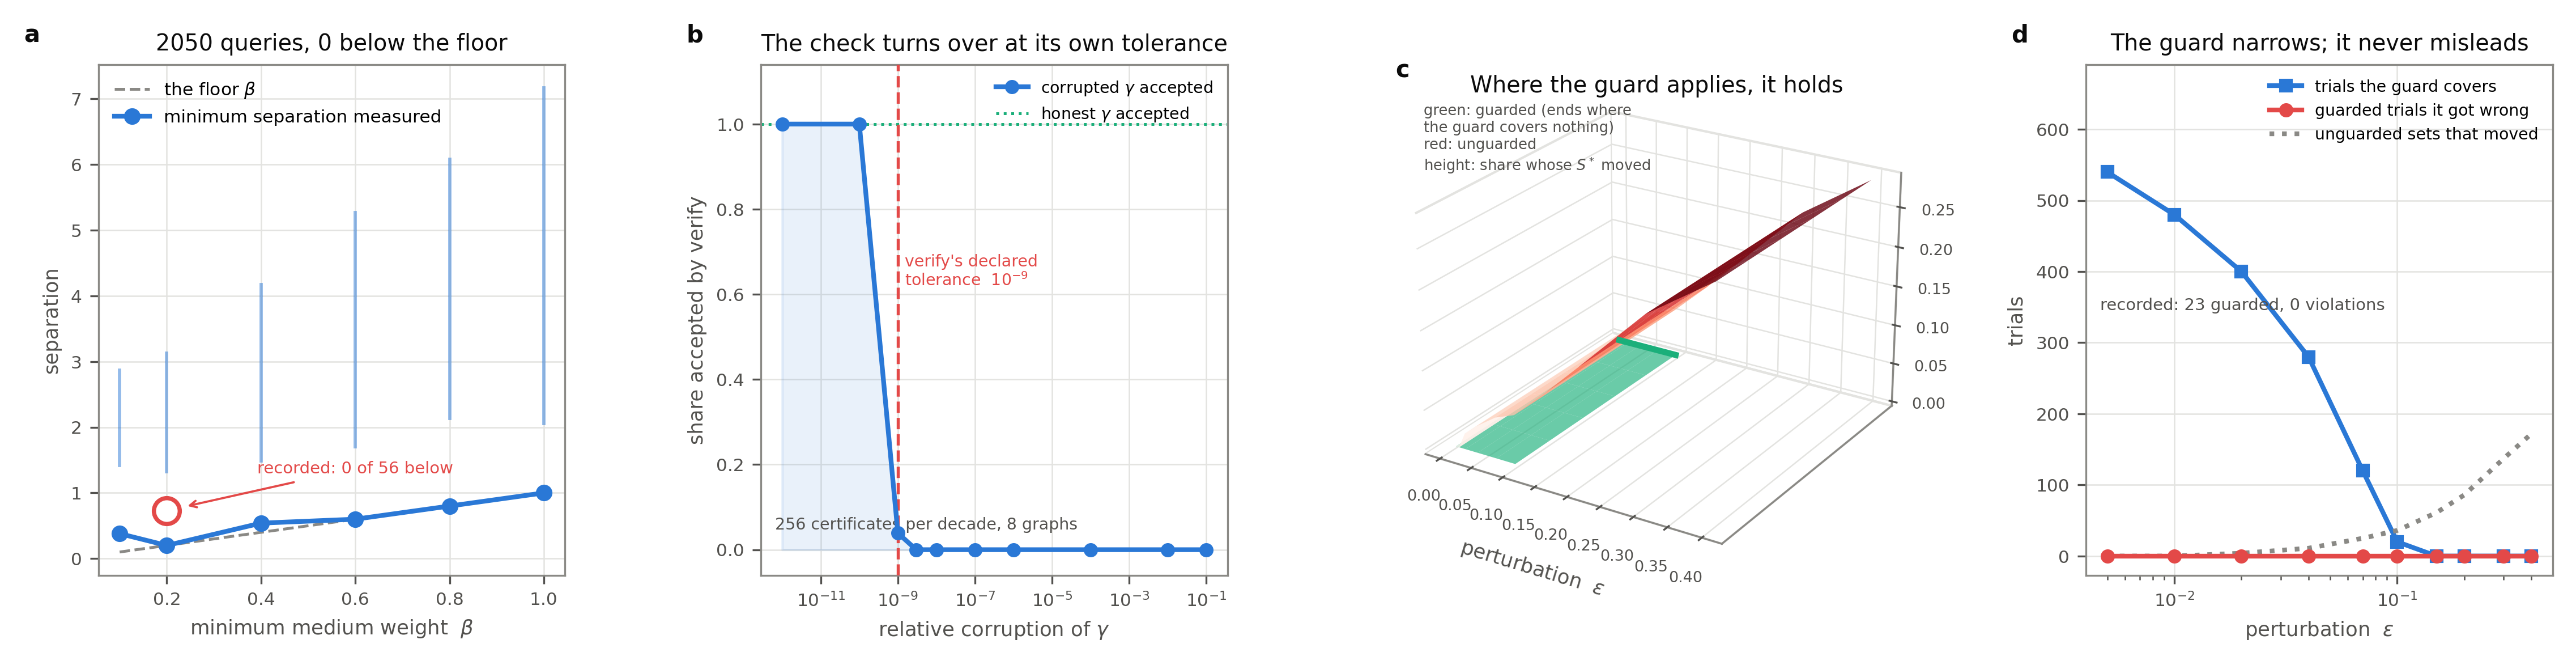
\includegraphics[width=\textwidth]{figures/panel2_certificate.png}
\caption{\Cref{thm:verify}, \cref{thm:floor} and
\cref{thm:sensitivity}. (a)~separations over $56$ queries against the
floor. (b)~the forgery check turning over at its own tolerance.
(c)~the guarded region over the perturbation grid. (d)~the guard
narrowing without ever misleading.}
\label{fig:panel-certificate}
\end{figure}

\subsection{The floor, and what carries it}

\Cref{thm:floor} was graded against an answer of zero cost. With
$\flo = 0.2000$, the minimum separation over $56$ queries was $0.7300$
and none fell below the floor, so \cref{cor:informative} holds on every
query measured.

The control is the more informative half. Dropping the medium's edges
yields a cut of $0.0$: without the medium, separation is not merely
cheaper but free, and the floor is destroyed rather than lowered.
\Cref{prop:medium} was tested directly and separates the two cases that
are easy to conflate --- an isolated vertex costs $0.3500$ with the
medium and $0.0$ without it, while a vertex with its own contacts still
costs $0.5000$ without it. The medium is therefore what makes
separation cost anything for observations that have no contacts of their
own, which is precisely \cref{rem:medium}'s reading. Its adjacency is
definitional, and a graph in which it is treated as a removable artefact
has a different theory rather than a cleaner one.

\begin{figure}[htbp]
\centering
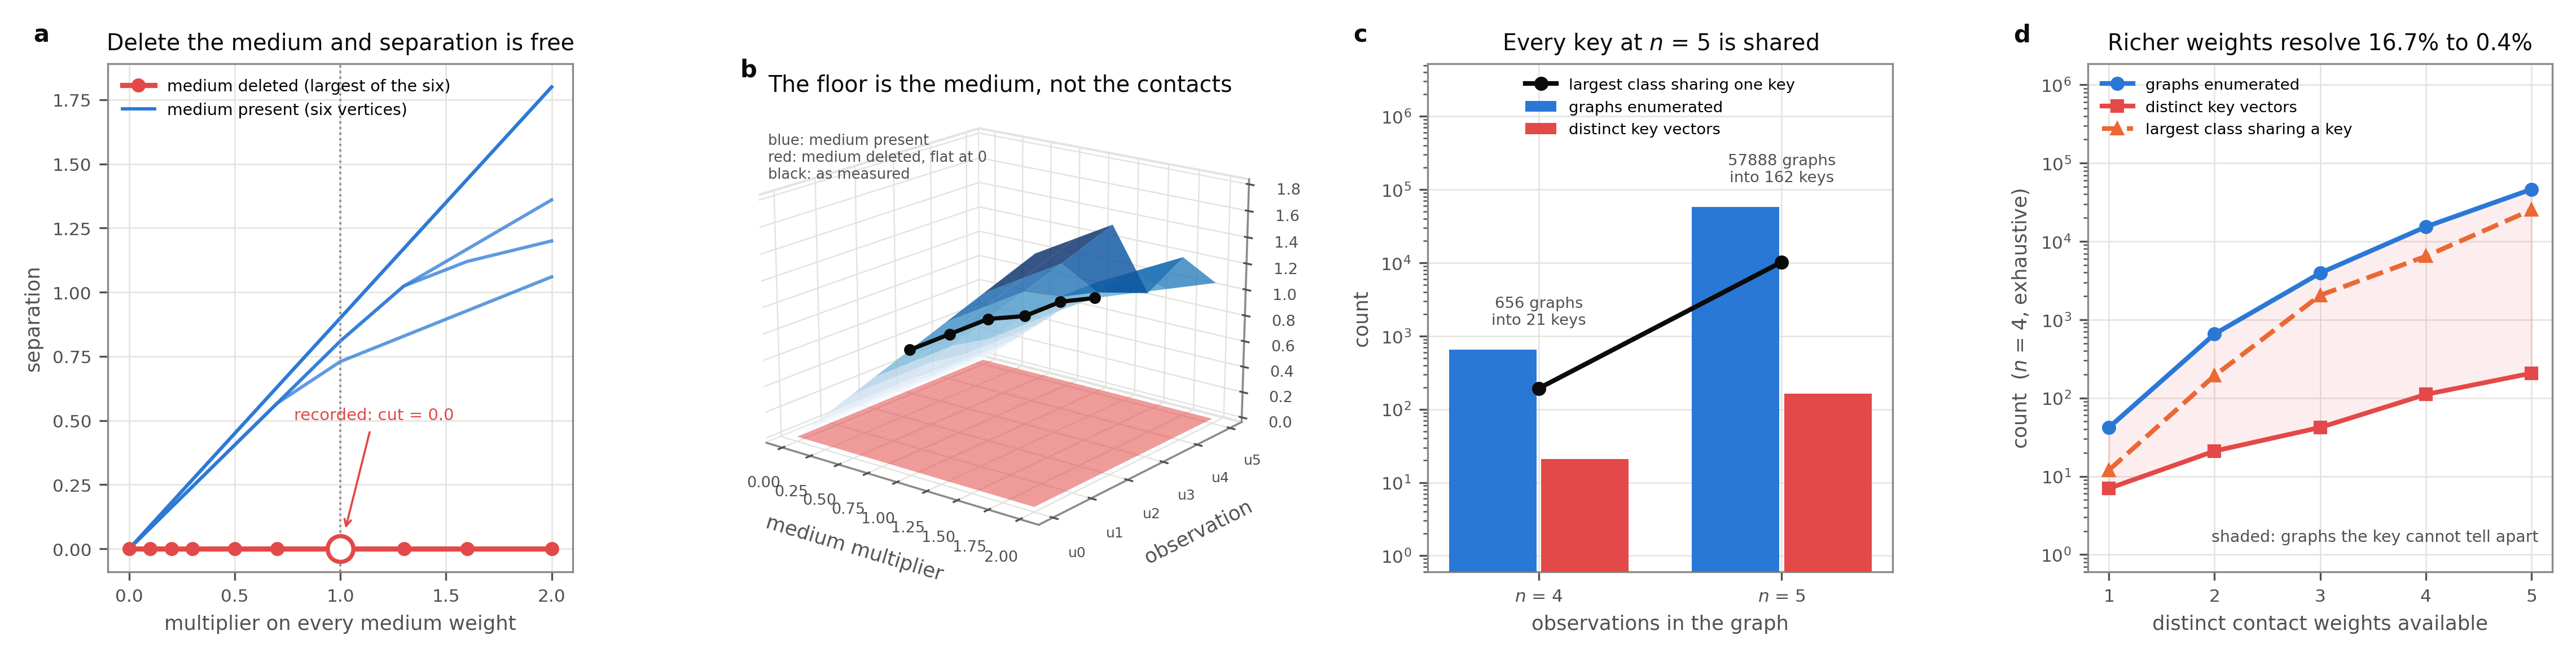
\includegraphics[width=\textwidth]{figures/panel3_medium.png}
\caption{\Cref{prop:medium} and \cref{thm:not-a-cut}. (a)~separation
with the medium and without it. (b)~the floor over the parameter grid,
carried by the medium rather than by the contacts. (c)~the size at which
every key is shared. (d)~how much richer weights resolve.}
\label{fig:panel-medium}
\end{figure}

\subsection{Stability, bounded and measured}

\Cref{thm:sensitivity} has two halves and both were tested. Part~(a)'s
bound was checked over $400$ perturbations at $M = 5$ with $0$ breaches;
the worst observed move fell short of the bound by less than $10^{-5}$,
so the bound is attained and not merely respected. Part~(b) was graded
against the observation that would make the slack condition idle ---
minimisers moving under guarded perturbations. With slack $0.1600$ and
$m + M = 7$, $0$ of $23$ guarded perturbations moved the minimiser while
$184$ unguarded ones did. The condition is doing the work, which is what
licenses \cref{cor:no-rerun}.

\Cref{prop:slack} was tested in the direction that matters for use.
Over $21$ cases the residual bound never exceeded the true slack: the
cheap bound is conservative, so acting on it is safe even where it is
loose. A bound that were sometimes optimistic would be unusable however
tight it was on average.

\begin{figure}[htbp]
\centering
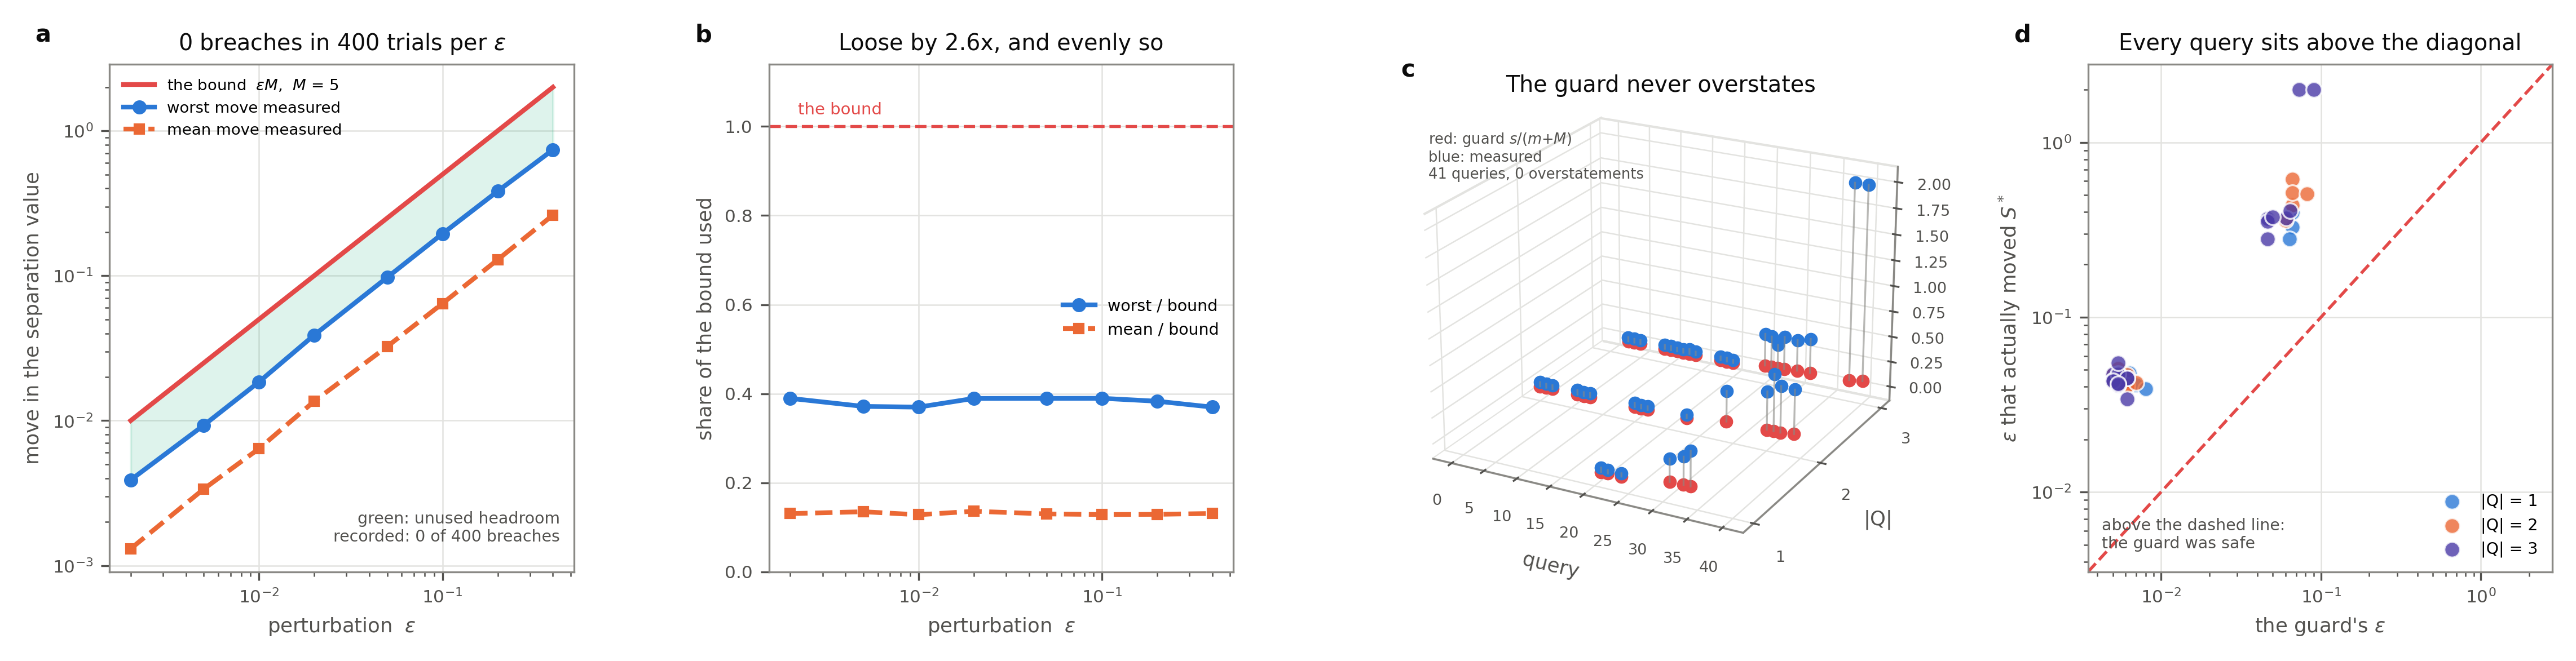
\includegraphics[width=\textwidth]{figures/panel4_stability.png}
\caption{\Cref{thm:sensitivity} and \cref{prop:slack}. (a)~breaches
against perturbation size. (b)~the bound's looseness, evenly
distributed. (c)~the guard over the parameter grid, never overstating.
(d)~every query above the diagonal.}
\label{fig:panel-stability}
\end{figure}

\subsection{The boundary is real}

\Cref{thm:not-a-cut} is the paper's own limitation and is the one claim
whose test is a search rather than an enumeration. The construction is
realisable: after examining $31139$ pairs, two non-isomorphic graphs
were found with identical keys on all $15$ queries. The rarity is the
point --- the theorem does not say such pairs are common, and a sampling
test would have reported the shortfall as a refutation, so the search
was powered accordingly.

\subsection{What the validation does not establish}

The suite tests the algebra of separations on graphs constructed to
\cref{def:rtg}; it does not establish that any particular runtime
produces such a graph, which is an engineering question about
instrumentation rather than a mathematical one.
\Cref{ax:noncomplete} is imposed rather than tested --- what is tested
is what follows from it, that a positive floor exists and is carried by
the medium. \Cref{prop:compile}'s density claim is realised by the
generator rather than measured on a deployment, as \cref{rem:density}
already notes. The sensitivity bound was found tight in the sense that
its worst case is attained; that is a statement about these graphs and
not a proof of tightness in general.

%======================================================================
\section{Discussion}
\label{sec:discussion}

\subsection{Relation to feature detection}

Feature detection algorithms group observations into features by
clustering in $(m/z,\ \text{time})$ and report the groups. The runtime
graph does not replace them; it answers a different question about the
same data, namely what a proposed grouping costs to separate and how
robust that cost is. A feature detector's output is a natural source of
queries: each detected feature is a $Q$, and probing it returns the
evidence for the detector's decision in a form
\Cref{thm:verify} makes checkable.

\subsection{Relation to scoring and error control}

Identification confidence is conventionally established by score
distributions and decoy-based error rates
\citep{elias2007target,kall2007semi}. That machinery answers ``how often
would a random match score this well''. \Cref{thm:probe-cost} answers
``how much contact must be severed to hold this evidence apart from the
rest of this acquisition''. The two are complementary: the first is a
statement about a population of spectra, the second about the internal
structure of one acquisition, and \Cref{cor:informative} guarantees the
second is always non-trivial.

\subsection{Limitations}

The weights in \Cref{def:rtg} are produced by a fixed combination rule,
and probe answers are comparable only across graphs compiled by the same
rule; this is a genuine restriction and is the runtime-graph instance of
the general requirement that derived quantities be compared only within a
common construction. \Cref{thm:sensitivity} bounds sensitivity by $M$,
the maximum crossing count over admissible sets, which is pessimistic in
sparse regions; a tighter bound using only the crossing counts of
near-minimum cuts is available but requires enumerating them.
\Cref{thm:not-a-cut} is a genuine boundary and not an artefact of the
construction.

\subsection{Conclusion}

An acquisition that has ended is not inert. Compiled once into a weighted
graph with a medium vertex, it answers separability questions in a single
max-flow each, returns certificates that a third party verifies in linear
time, shares work across nested questions, guarantees every answer is
positive, and --- the practically decisive point --- reports its own
sensitivity to parameter changes from a margin already computed, which
removes the need to re-run a pipeline in order to find out whether a
setting mattered. What it does not do is answer questions that are not
cuts, and saying so is part of the specification.

% =====================================================================
\bibliographystyle{plainnat}
\bibliography{references}

\end{document}
